\section{Introduction}

This exposition gives an overview of the Elmer software package. General information 
on the capabilities of the software, its usage, and how the material of the package 
is organized is presented. More detailed information is given
in the other Elmer manuals, the scopes of which are described in this document.
%The emphasis is on the total view
%and the user is encouraged to read the other Elmer manuals for more detailed information. 

\subsection*{What is Elmer}

Elmer is a finite element software package for the solution of partial differential 
equations. Elmer can deal with a great number of different equations, which may be coupled 
in a generic manner making Elmer a versatile tool for multiphysical simulations. 
As an open source software, Elmer also gives the user the means to modify the existing 
solution procedures and to develop new solvers for equations of interest to the user.  

\subsection*{History of Elmer}
The development of Elmer was started in 1995 as part of a national CFD technology 
program funded by the Finnish funding agency for technology and innovation, Tekes. 
The original development consortia included partners from CSC -- IT Center 
for Science (formely known as CSC -- Scientific Computing), Helsinki University of Technology TKK, VTT Technical Research Centre of Finland,
University of Jyv�skyl�, and Okmetic Ltd. After the five years initial project ended 
the development has been continued by CSC in different application fields.

\subsection*{Licensing}
In September 2005 Elmer was released under GNU General Public License (GPL). This 
has widened the user community, particularly the number of international users has grown.
However, as the sole owner of the copyright to Elmer source code, CSC may distribute 
Elmer also under other licensing terms. Therefore, if GPL does not suit your purposes, 
you may contact the Elmer team for other licensing options. 

\subsection*{Distribution}
Elmer is distributed only through the Internet. The actual distribution site may vary 
but the pointer to the location may always be found at \URL{http://www.csc.fi/elmer}. 

The distribution of Elmer comes in three different parts: sources, binaries, and documentation.
Unix users are encouraged to 
compile the software themselves. The compilation instructions are given at the www-page.
For Windows and Macintosh a precompiled binary version of the code is also provided. 
The documentation of the software is already quite extensive, but unfortunately still not complete.

\subsection*{Contributing}
Everybody is welcome to contribute to the Elmer project. 
Often the bottle-neck is in case specification, testing and verification which may be done 
without in-depth knowhow of the code. Also contributions to the code are welcome. However, before 
granting a permission to commit to the main source file archive a Elmer Contributor Agreement 
has to be signed. This gives CSC the right to use contributions to Elmer under the current free software license, 
and also under other licenses we may use. However, this does not limit the contributors right to use the contributed code
in any way. 


\section{Key features of Elmer}

Elmer offers a wide range of methods and techniques for the computational modeling of
physical phenomena described by partial differential equations.
In the following some of the most essential ones are summarized.

\subsection*{Physical models in Elmer}
The Elmer package contains solvers for a variety of mathematical models.
The following list summarizes the capabilities of Elmer in specialized fields.
\begin{itemize}
  \item Heat transfer: models for conduction, radiation and phase change
  \item Fluid flow: the Navier-Stokes, Stokes and Reynolds equations, k-$\varepsilon$ model
  \item Species transport: generic convection-diffusion equation
  \item Elasticity: general elasticity equations, dimensionally reduced models for plates and shells
  \item Acoustics: the Helmholtz equation
  \item Electromagnetism: electrostatics, magnetostatics, induction
  \item Microfluidics: slip conditions, the Poisson-Boltzmann equation
  \item Levelset method: Eulerian free boundary problems 
  \item Quantum Mechanics: density functional theory (Kohn-Sham)
\end{itemize}

\subsection*{Numerical methods in Elmer}

For approximation and linear system solution Elmer offers a great number of possibilities.
The following list summarizes some of the most essential ones.

\begin{itemize}
  \item All basic element shapes in 1D, 2D and 3D with the Lagrange shape functions
of degree $k \le 2$
  \item Higher degree approximation using $p$-elements
  \item Time integration schemes for the first and second order equations
  \item Solution methods for eigenvalue problems
  \item Direct linear system solvers (Lapack \& Umfpack)
  \item Iterative Krylov subspace solvers for linear systems
  \item Multigrid solvers (GMG and AMG) for some basic equations
  \item ILU preconditioning of linear systems
  \item Parallelization of iterative methods
  \item The discontinuous Galerkin method
  \item Stabilized finite element formulations, including the methods of residual free bubbles and SUPG
  \item Adaptivity, particularly in 2D 
  \item BEM solvers (without multipole acceleration)
\end{itemize}

\subsection*{Pros and Cons of Elmer}
Potential users may find a list of the possible pros and cons of Elmer package useful.
The following summary is naturally open to subjective judgment and not complete either.
\begin{itemize}
\item[+] Since Elmer is an open source product, it is possible to verify and modify the solution procedures
\item[+] Elmer has a modern programmable graphical user interface 
\item[+] Elmer can handle the coupling of field equations in a flexible manner and new field variables can be 
  introduced easily
\item[+] All material parameters may depend on the field variables and other parameters in a free manner
\item[+] Elmer offers a large selection of modern numerical methods
\item[+] Elmer enables the user to use most generally used finite elements
\item[+] Assembly and iterative solution can also be done in parallel
\item[+] Elmer has a graphical preprocessing interface for simple problem setups
\item[+] Elmer is easily compiled for most Unix systems and it is also available
  for Windows and Macintosh machines as precompiled binaries
\item[+] Elmer has a steadily growing user community and it has already been used in tens of 
   scientific papers 
\item[-] The different aspects of the code (solver, interface, documentation) are not always at the same 
development phase. For example documentation is not up-to-date and interface lacks many of the more esoteric
physical models provided by the solver. 
\item[-] Getting acquainted with the large package may take time. Previous experience on FEM packages 
  may therefore be useful.
\item[-] Elmer itself does not include proper geometry or mesh generation tools for geometrically 
  complicated problems. Only mesh import interfaces are supported.
\item[-] As a multiphysical solver Elmer may sometimes lack features in some areas that are standard for
	established single-field codes. 
         Thus, some users may find the capabilities of Elmer inadequate for their needs. 
\end{itemize}





\section{Elmer executables}

As most finite element packages, Elmer is divided into a number of separate
executables that may also be used independently. The main parts are the preprocessor, solver
and postprocessor, but there are also other modules that may be called for specific assignments. 

\sifbegin
\sifitem{ElmerGUI}{}
ElmerGUI is the new graphical user interface for Elmer software
based on the Qt cross-platform application framework (see. http://trolltech.com/products/qt/). 
ElmerGUI includes elmergrid, and optionally tetlib and nglib,
as finite element mesh generators. ElmerGUI does not include any geometry definition tools so for defining the 
original geometry some other software must be used. However, the large number of supported formats should make
the mesh import straight-forward. With ElmerGUI the problem setup may be done easily using programmable 
menu structures that make the modification of the GUI very simple. ElmerGUI also controls the ElmerSolver and 
ElmerPost binaries and includes a real-time convergence monitor. ElmerGUI is still in its early development 
phase as the development was started in early 2008. 


\sifitem{ElmerSolver}{}
ElmerSolver is a program executable forming the solver of Elmer. 
It is the soul of the Elmer software and the part where most of the development work is 
directed to. ElmerSolver includes a large number of finite element library tools
which enable the user to write new equation solvers economically. The specific equation
solvers are mainly available as dynamical libraries that have standard interfaces and can
be linked to the main program on request. 

\sifitem{ElmerPost}{}
ElmerPost is a versatile postprocessor that is expected to be quite sufficient for the 
usual postprocessing needs. ElmerPost provides a straightforward graphical user interface 
that is easy to learn. ElmerPost utilizes Mesa and TCL/TK graphics libraries. 

\sifitem{ElmerGrid}{}
ElmerGrid provides functionality for the generation of simple structured meshes and may also be used 
for mesh manipulation and transformation tasks of many kinds. For example, ElmerGrid may be used
to partition the mesh for parallel runs or to import meshes written by other mesh generators. 
The ElmerGrid command file is to be written by a text editor. 

\sifitem{ElmerFront}{}
ElmerFront is the old graphical user interface for creating setups for simple problems. 
ElmerFront is not actively developed and therefore a large part of the functionality of ElmerSolver
is not supported by ElmerFront. The meshing capabilities of ElmerFront are limited to 
two-dimensional meshes of the Delaunay type, which are obtained by calling \texttt{Mesh2D} program. 
ElmerFront will still be distributed but it is no longer supported in any way and hence it will with
time become obsolite. The replacement of ElmerFront is ElmerGUI. 

\sifitem{Mesh2D}{}
This is a Delaunay triangulator that is called by ElmerFront but it may also be called independently.

\sifitem{ViewFactors}{}
This is a program for the computation of view factors that need to be determined in some radiation 
problems. Usually there is no need to call this independently as it is automatically called 
within ElmerSolver.
\sifend



\section{Elmer source code}

Elmer development uses the subversion version control system available at sourceforge. 
The code may be viewed under "Code" and you may obtain a complete snapshot of the source codes, for example with
\begin{verbatim}
  svn co https://elmerfem.svn.sourceforge.net/svnroot/elmerfem elmerfem
\end{verbatim}
This is the recommended way of obtaining the source codes since it is always up to date. 

Elmer source code is also available 
as tar bundles bearing the suffix \texttt{tar.gz} in the following sites
\begin{verbatim}
  http://www.nic.funet.fi/pub/sci/physics/elmer/src
  http://sourceforge.net/projects/elmerfem
\end{verbatim}
The numbering of the tar bundles indicates to which version of Elmer the source is related to. 
The first version number is changed in 
major new releases, while the last-named version numbers indicate minor changes taking place few times in a year. 

Elmer is distributed as partially interdependent modules. Some of them are used for creating
program executables while others are only used for creating program libraries. 
Basically knowing the module interdependencies is unnecessary unless the user wants to 
setup only a partial system.

\sifbegin
\sifitem{eio}{}
Elmer input/output library written in C++ and used for some I/O operations by the ElmerSolver. 
\sifitem{elmergrid}{}	
ElmerGrid source codes written in C, including also the Metis library from the Karypis Lab. 
\sifitem{elmerpost}{} 	
ElmerPost source codes written in C. 
\sifitem{fem}{}	
ElmerSolver source codes written mainly in Fortran90.
\sifitem{front}{}
ElmerFront source codes written in C++.
\sifitem{hutiter}{} 
The iterative linear algebra solvers written mainly in Fortran90 and called by ElmerSolver.
\sifitem{matc}{} 
This library is used in the command file interpreter of ElmerSolver and inside the command 
window of ElmerPost for evaluating mathematical expressions written in C.  
\sifitem{mathlibs}{}	
This includes basic mathematical libraries such as Lapack, Blas, Arpack, and Parpack.
\sifitem{meshgen2d}{} 
This includes the source code of the 2D Delaunay mesher. 
\sifitem{misc}{}
Miscallenous developments, also the new preprocessor ElmerGUI may be found here under the directory Mesh3D. 
\sifitem{umfpack}{}
This includes the source code of the Umfpack (GPL version 4.4) library from University of California.
\sifend


\section{Elmer documentation}

The Elmer documentation is constantly under development. The date of the manual version is 
printed in the cover of the manual. The current set of Elmer manuals is as follows.

\sifbegin
\sifitem{ElmerSolverManual.pdf}{}
	ElmerSolver Manual gives an overview of the general capabilities of the solver,
        focusing on the utilities that are of use to several physical models. It follows 
        from this organization of material that information specific to a certain physical 
        model is not included in this manual.
\sifitem{ElmerModelsManual.pdf}{}
	The Models Manual describes the different physical models which the solver of Elmer can handle.
        The specific options for controlling the corresponding equation solvers are also documented. 
        In addition, this manual describes certain utilities for other tasks, such as computing
        derived quantities.  
\sifitem{ElmerTutorials.pdf}{}
	The tutorials of the Elmer software are basically just example files with documentation.
        The files related to the tutorials are contained in 
	\texttt{ElmerTutorialFiles.tar.gz} which can be found at the same site where the manuals
        are located.
\sifitem{ElmerGridManual.pdf}{}
	This is the manual of ElmerGrid utility. The
	examples related to the ElmerGrid documentation are provided in the file 
	\texttt{ElmerGridExamples.tar.gz} which can be found at the same site where the manuals
        are located.
\sifitem{ElmerFrontUserGuide.pdf}{}
	This is the manual for the graphical user interface ElmerFront. ElmerFront is not actively developed 
	and this might be the final documentation of the program.
\sifend
In addition to these manuals there are separate documentation for some input interfaces (GiD) and
for visualization tasks (making animations). Look at the www-pages for more information on these
documents. Some useful information may also be found in the following old documents.
\sifbegin
\sifitem{OldElmerUserGuide.pdf}{}
	This is the original user guide of Elmer software (1999). Particularly some appendices 
        defining some of the file formats may still be useful.
\sifitem{OldElmerTutorial.pdf}{}
	A graphical user interface oriented tutorial guide of the Elmer software (2000). 
\sifend





%\begin{figure}[tbhp]
%\vspace{-20mm}
%\begin{center}
%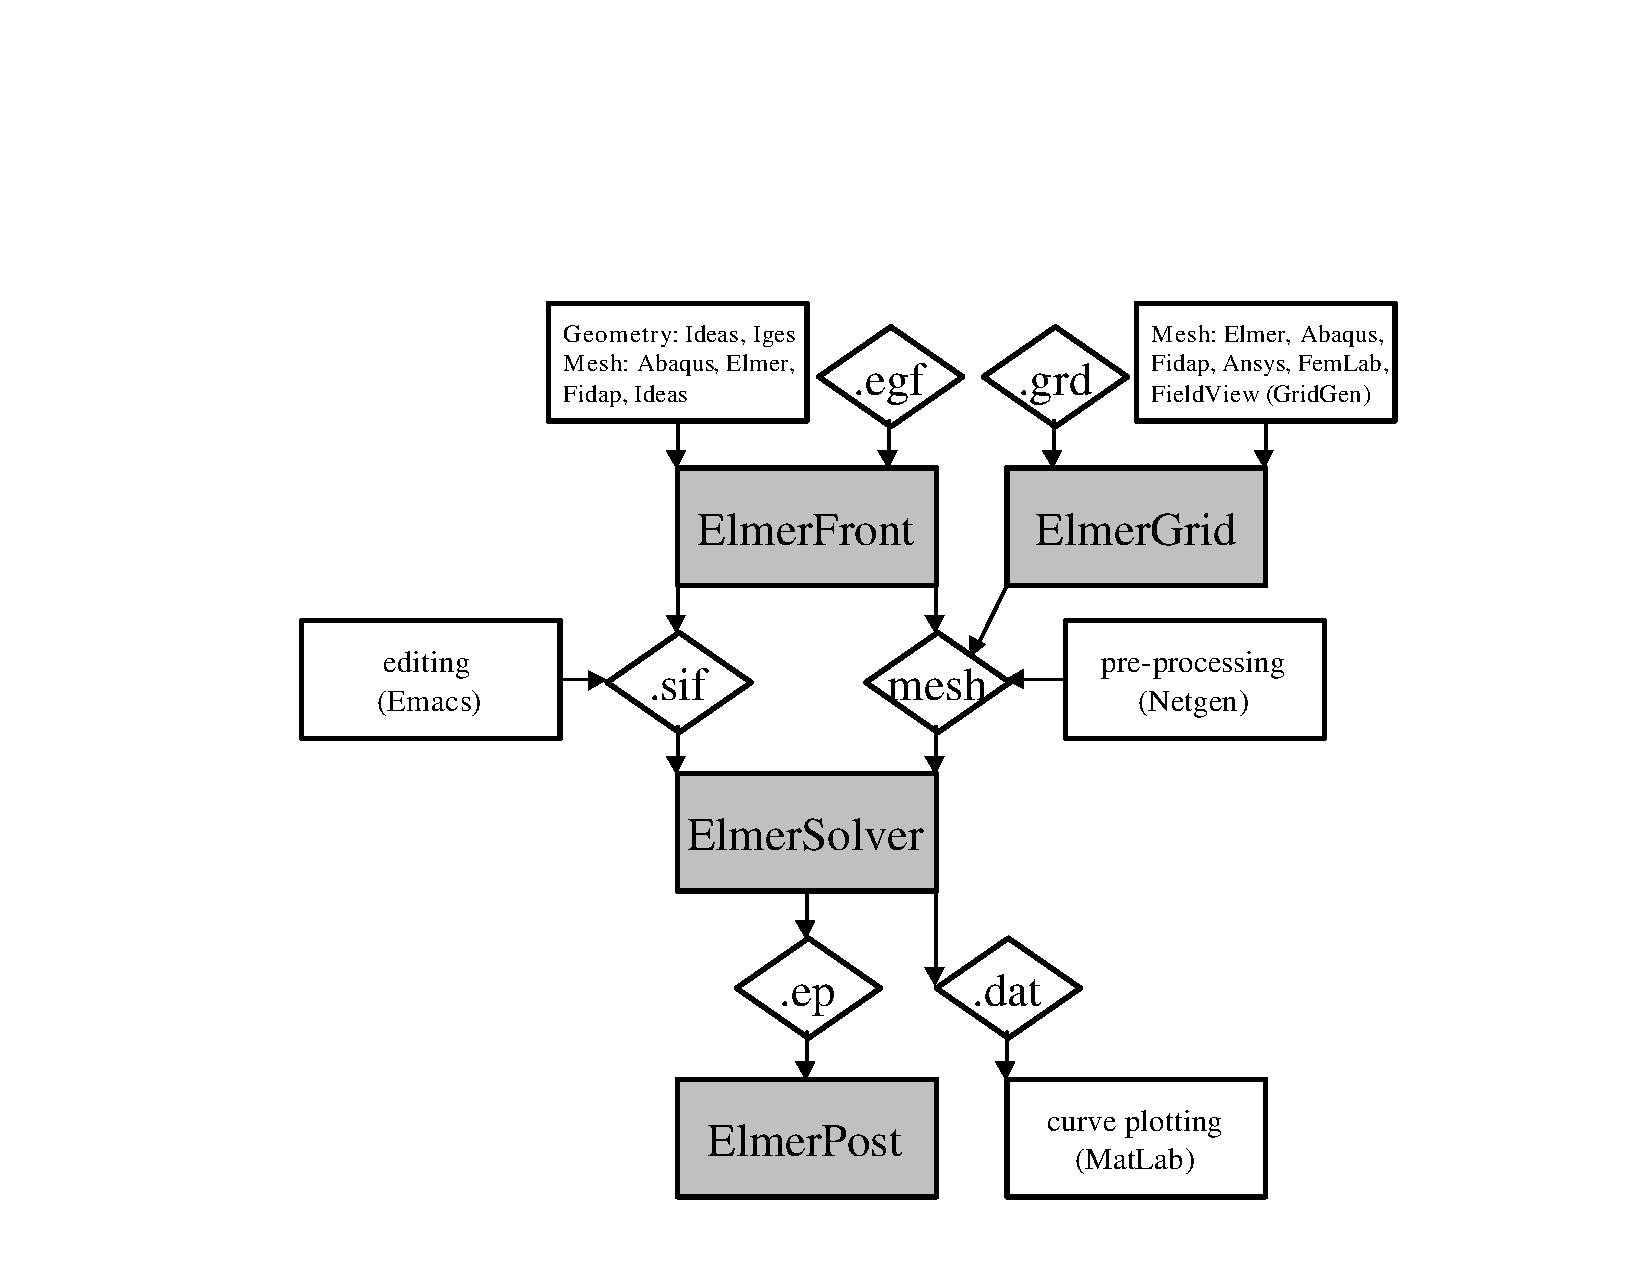
\includegraphics[width=13.0cm]{elmer-chart.pdf}
%\caption{Work flow in the Elmer environment}
%\label{fig_workflow}
%\end{center}
%\end{figure}



\section{Strategies for using the Elmer package}

The modularity of the Elmer package enables the users to have different strategies 
for using Elmer. 
%
%Figure~\ref{fig_workflow} shows schematically how the key
%software components depend on one another. 
%
Here the possible ways of using
the package are outlined. How the input and output data of the software components
are organized into files is also summarized.



\subsection{Elmer file system}

The following list summarizes how the input and output data are organized into files.

%\section{Elmer file formats}
%Elmer uses and creates variable number of files in the solution of the case. 
%Here is some information about the Elmer file system. 

\sifbegin
\sifitem{ElmerSolver command file}{*.sif}
The file with the sif-suffix is the command file which is read by ElmerSolver.
It contains user-prepared input data that controls the selection of physical models,
boundary conditions, and so on. In the case of simple problem setups this command file 
may be written automatically by ElmerFront. More complicated setups require that this 
file is edited using a text editor. The documentation of the software includes several
example files that may be used as starting points when editing the command file.
For the keyword syntax of the command file
the ElmerSolver Manual and Models Manual are the best sources of information.

\sifitem{ElmerSolver mesh files}{mesh.*}
The solver of Elmer reads the mesh from four different files \texttt{mesh.nodes},
~\texttt{mesh.elements},\linebreak[4] \texttt{mesh.boundary}, and \texttt{mesh.header},
which all should be located in a single mesh directory. The mesh files may be created using 
ElmerFront, ElmerGrid, or by enhanced versions of Netgen and GiD. A program executable
Mesh2D which is the mesh generator used by ElmerFront may also be called independently.
The file format of the mesh files is compatible with ElmerSolver, ElmerFront and ElmerGrid.

\sifitem{ElmerSolver result file}{*.result}
This result file is written by ElmerSolver and may be used to make a simulation 
restart from a previous set of results. ElmerSolver by default writes this file to 
the mesh directory. The file format is compatible only with ElmerSolver.

\sifitem{ElmerPost file}{*.ep}
This file is written by ElmerSolver and can be read by ElmerPost. 
ElmerSolver by default writes this file to the mesh directory.
The file is used mainly for visualization purposes.

\sifitem{ElmerGrid mesh definition file}{*.grd}
This file is used to define 1D, 2D or 3D structured meshes. 
The file can only be read by ElmerGrid.

\sifitem{ElmerGrid command file}{*.eg}
This file is used to make mesh manipulation operations with ElmerGrid. The same functionality 
may be achieved by using command line arguments.

\sifitem{ELMERSOLVER\_STARTINFO}{} 
This file is used by ElmerSolver and simply includes the name of the command file.
The other possibility to transfer the command file name to ElmerSolver is to use 
a command line parameter.

\sifitem{SOLVER.KEYWORDS}{}
The keywords that may be used in the ElmerSolver command file are listed in this file, located 
in the directory of the shared library files of ElmerSolver. This list may not be complete as new keywords 
are always popping up due to the development work. Therefore the user may create a local file and 
add the missing keywords to this file. Note that it does not really matter if a keyword is not listed
as long as the type of the keyword value is given in the command file and ElmerSolver is not asked to
do a strict checking of keywords. 
%; see the documentation of the \texttt{check keywords warn} keyword.
%in the command file the \texttt{Check Keywords Warn} is used 
%instead of \texttt{abort}. 

\sifitem{Elmer geometry file}{*.egf}
This file defines a 2D geometry using primitives such as points and lines.
It is read by the ElmerFront program and can be edited using a text editor.

\sifitem{Elmer mesh generator input file}{*.mif}
This is the file that Mesh2D uses to create Delaunay triangulations. 
It is usually written by ElmerFront but it may easily be modified using an editor.


\sifend 


\subsection{Strategies for preprocessing}

The purpose of the preprocessing phase is to create the ElmerSolver input files, which 
are at the minimum the command file and the mesh files. Before the introduction of ElmerGUI
the strategies for using Elmer were rather mixed since power users tended to avoid ElmerFront
which was still used by many in the introductory phase. It is hoped that with the ElmerGUI
the different strategies will be more unified. 


\subsubsection*{Existing mesh definition file + ElmerGUI}

ElmerGUI includes 
ElmerGrid, and optionally tetlib and nglib,
as finite element mesh generators.
When a suitable mesh definition file for these software exists the mesh is created on-the-fly
before reading it into ElmerGUI. ElmerGUI can also be used to pass inline parameters to the mesh
generators which often allows sufficient control over the mesh generators. However, full control 
of the mesh generation process with complicated geometries is not possible with the provided interface.
However, still this approach provides maybe the easiest way to start using Elmer. 


\subsubsection*{Existing mesh + ElmerGUI}

ElmerGUI is also able to read many existing mesh formats. These include .FDNEUT (Gambit), 
.msh (gmsh), .mphtxt (Comsol Multiphysics), and .unv (Ideas universal) file formats. 
Additionally there is a small number of third party mesh generators that can directly write meshes in Elmer format
provided that some interfaces are used. Currently interfaces for GiD and Netgen are provided. 
For more information on the interfaces see the Elmer www-pages. 
This approach is not limited by the mesh generation possibilities of ElmerGUI and is therefore suitable 
even for the most complicated cases, provided that a good mesh generation software is at disposal.


\subsubsection*{Existing mesh and command file + editor}

ElmerGUI is often used as the first-step tool in the simulations. However, if in following simulations only minor
modifications to the initail setup are needed it is often most practical to edit the command file 
(*.sif) by some text editor (e.g. emacs). A good place to start may be one of the minimal test cases 
provided in the source distribution. The more than one hundred tests ofetn provides a close-enough starting point
for consecutive simulations particularly if the geometry is rather simple.
Also it may be that some new solvers are not implemented in the 
ElmerGUI and hence adding the manually is the only option. 
In adding the keywords in the
command file, the Models Manual is of great help. In this approach ElmerSolver and ElmerPost 
are to be executed from the command line. 


\subsubsection*{ElmerGrid + editor}

An easy way to make simple 2D and 3D meshes is to use ElmerGrid. The mesh definition file 
of ElmerGrid also defines the geometry. However, the structured format of ElmerGrid favors
box-like forms and making more complicated shapes may be difficult. 
In this approach 
the solver command file must be created using a text editor. Previous command files provide a good 
starting point also in this case. 

This approach is most suited for making academic tests using simple structured meshes. 
It is easy to test different things in this approach as the mesh is basically fully parameterized. 
Many of the provided tests of ElmerSolver are defined using this approach. 
Trying to push this approach to more complicated shapes may turn out to be cumbersome. 
 
Sometimes ElmerGrid needs also to be used as on intermediate tool, for example in the partitioning of the mesh.
Then the changes to the command file are often quite minimal. 


\subsubsection*{Geometry definition or mesh + ElmerFront}

For users accustomed to ElmerFront it may still provide a good alternative for performing the simulations.
However, new users are not recommended to follow this paty. 

In ElmerFront the mesh may be either defined using the built-in mesh generation tool, Mesh2D, or 
reading in an existing mesh in some of the supported formars (Abaqus, Fidap, Ideas, Elmer). 
After reading the geometry data or mesh,
ElmerFront may be used to (create the mesh and) define the equations, boundary and initial conditions, 
and material parameters. The functionality of ElmerFront is not actually limited to 
preprocessing tasks, since the program executables for the solution and the visualization of the results 
(ElmerSolver and ElmerPost) can also be started via ElmerFront.

A handicap with ElmerFront is that it does not have any geometry definition tools,
and the mesh generation tools are limited to 2D Delaunay. In addition,
a large portion of the capabilities of ElmerSolver are not supported by ElmerFront. 
Therefore using ElmerFront as the only strategy is best suited for relatively simple tasks 
with some standard equations (heat, flow, stress). The benefit of this approach 
is that the user does not need to get acquainted with the different file formats, 
nor edit the files by hand. However, serious users have to abandon this approach as the only strategy quite soon. 




\subsection{Strategies for postprocessing}

There are also several strategies for visualizing the numerical results.

\subsubsection*{ElmerPost}
The easiest way for visualization is to use ElmerPost. ElmerPost does not pose any severe limitations 
and has good features in exporting data in raster formats or animations.
However, if you want to draw line graphs, or want to have several data sets available at the same
time, you need other file formats as well. 

\subsubsection*{VTK, GiD etc.}
ElmerSolver can write the results also in formats understood by some third party visualization 
software. Use the \texttt{ResultOutputSolve} keyword (see Elmer Models Manual) for outputting 
in VTK (Visit, Paraview,\ldots ) or GiD format.

\subsubsection*{Matlab, gnuplot, etc.}
Ascii data for producing line graphs can be written automatically by saving the 
solution data along predefined lines, or lines that are created on-the-fly.
For this purpose use the \texttt{SaveScalars} or \texttt{SaveLine} keyword (see Elmer Models Manual).


\section*{Contact info}

For questions concerning the use and capabilities of Elmer, 
please use preferably the Elmer discussion mailing list at \texttt{elmerdiscussion@postit.csc.fi}.

%\mbox{}\newline\noindent
%You can contact also directly some of the Elmer developers:
%\begin{itemize}
%\item Lyly Mikko, mikko.lyly@csc.fi
%\item Mika Malinen, mika.malinen@csc.fi
%\item Pursula Antti, antti.pursula@csc.fi
%\item Ruokolainen Juha, juha.ruokolainen@csc.fi
%\item R�back Peter, peter.raback@csc.fi
%\end{itemize}